
\documentclass[letterpaper,hide notes,xcolor={table,svgnames},pdftex,10pt]{beamer}
\def\showexamples{t}

\usecolortheme{crane}
\setbeamertemplate{navigation symbols}{}

\usetheme{MyPittsburgh}
\usepackage{hyperref}
\usepackage{graphicx,xspace}
\usepackage[normalem]{ulem}
\usepackage{multicol}
\usepackage{amsmath,amssymb,amsthm,graphicx,xspace}
\newcommand\SF[1]{$\bigstar$\footnote{SF: #1}}

\usepackage[sfdefault,lf]{carlito}
\usepackage[T1]{fontenc}
\usepackage[scaled]{beramono}
\usepackage{tikzpagenodes}
\newcommand{\Rplus}{\protect\hspace{-.1em}\protect\raisebox{.35ex}{\small{\small\textbf{+}}}}
\newcommand{\Cpp}{\mbox{C\Rplus\Rplus}\xspace}

\newcounter{tmpnumSlide}
\newcounter{tmpnumNote}

\newcommand\mnote[1]{%
	\addtocounter{tmpnumSlide}{1}
	\ifdefined\showcues {~\tiny\fbox{\arabic{tmpnumSlide}}}\fi
	\note{\setlength{\parskip}{1ex}\addtocounter{tmpnumNote}{1}\textbf{\Large \arabic{tmpnumNote}:} {#1\par}}}

\newcommand\mmnote[1]{\note{\setlength{\parskip}{1ex}#1\par}}


\newcommand\mquestion[2]{{~\color{red}\fbox{?}}\note{\setlength{\parskip}{1ex}\par{\Large \textbf{?}} #1} \note{\setlength{\parskip}{1ex}\par{\Large \textbf{A}} #2\par}\ifdefined \presentationonly \pause \fi}

\newcommand\blackboard[1]{%
	\ifdefined   \showblackboard
		{#1}
	\else {\begin{center} \fbox{\colorbox{blue!30}{%
						\begin{minipage}{.95\linewidth}%
							\hspace{\stretch{1}} Some space intentionally left blank; done at the blackboard.%
						\end{minipage}}}\end{center}}%
	\fi%
}

\usepackage{listings}
\lstset{%
	keywordstyle=\bfseries,
	aboveskip=15pt,
	belowskip=15pt,
	captionpos=b,
	identifierstyle=\ttfamily,
	frame=lines,
	numbers=left, basicstyle=\scriptsize, numberstyle=\tiny, stepnumber=0, numbersep=2pt}

\usepackage{siunitx}
\newcommand\sius[1]{\num[group-separator = {,}]{#1}\si{\micro\second}}
\newcommand\sims[1]{\num[group-separator = {,}]{#1}\si{\milli\second}}
\newcommand\sins[1]{\num[group-separator = {,}]{#1}\si{\nano\second}}
\sisetup{group-separator = {,}, group-digits = true}

%% -------------------- tikz --------------------
\usepackage{tikz}
\usetikzlibrary{positioning}
\usetikzlibrary{arrows,backgrounds,automata,decorations.shapes,decorations.pathmorphing,decorations.markings,decorations.text}

\tikzstyle{place}=[circle,draw=blue!50,fill=blue!20,thick, inner sep=0pt,minimum size=6mm]
\tikzstyle{transition}=[rectangle,draw=black!50,fill=black!20,thick, inner sep=0pt,minimum size=4mm]

\tikzstyle{block}=[rectangle,draw=black, thick, inner sep=5pt]
\tikzstyle{bullet}=[circle,draw=black, fill=black, thin, inner sep=2pt]

\tikzstyle{pre}=[<-,shorten <=1pt,>=stealth',semithick]
\tikzstyle{post}=[->,shorten >=1pt,>=stealth',semithick]
\tikzstyle{bi}=[<->,shorten >=1pt,shorten <=1pt, >=stealth',semithick]

\tikzstyle{mut}=[-,>=stealth',semithick]

\tikzstyle{treereset}=[dashed,->, shorten >=1pt,>=stealth',thin]

\usepackage{ifmtarg}
\usepackage{xifthen}
\makeatletter
% new counter to now which frame it is within the sequence
\newcounter{multiframecounter}
% initialize buffer for previously used frame title
\gdef\lastframetitle{\textit{undefined}}
% new environment for a multi-frame
\newenvironment{multiframe}[1][]{%
	\ifthenelse{\isempty{#1}}{%
		% if no frame title was set via optional parameter,
		% only increase sequence counter by 1
		\addtocounter{multiframecounter}{1}%
	}{%
		% new frame title has been provided, thus
		% reset sequence counter to 1 and buffer frame title for later use
		\setcounter{multiframecounter}{1}%
		\gdef\lastframetitle{#1}%
	}%
	% start conventional frame environment and
	% automatically set frame title followed by sequence counter
	\begin{frame}%
		\frametitle{\lastframetitle~{\normalfont(\arabic{multiframecounter})}}%
		}{%
	\end{frame}%
}
\makeatother

\makeatletter
\newdimen\tu@tmpa%
\newdimen\ydiffl%
\newdimen\xdiffl%
\newcommand\ydiff[2]{%
	\coordinate (tmpnamea) at (#1);%
	\coordinate (tmpnameb) at (#2);%
	\pgfextracty{\tu@tmpa}{\pgfpointanchor{tmpnamea}{center}}%
	\pgfextracty{\ydiffl}{\pgfpointanchor{tmpnameb}{center}}%
	\advance\ydiffl by -\tu@tmpa%
}
\newcommand\xdiff[2]{%
	\coordinate (tmpnamea) at (#1);%
	\coordinate (tmpnameb) at (#2);%
	\pgfextractx{\tu@tmpa}{\pgfpointanchor{tmpnamea}{center}}%
	\pgfextractx{\xdiffl}{\pgfpointanchor{tmpnameb}{center}}%
	\advance\xdiffl by -\tu@tmpa%
}
\makeatother
\newcommand{\copyrightbox}[3][r]{%
	\begin{tikzpicture}%
		\node[inner sep=0pt,minimum size=2em](ciimage){#2};
		\usefont{OT1}{phv}{n}{n}\fontsize{4}{4}\selectfont
		\ydiff{ciimage.south}{ciimage.north}
		\xdiff{ciimage.west}{ciimage.east}
		\ifthenelse{\equal{#1}{r}}{%
			\node[inner sep=0pt,right=1ex of ciimage.south east,anchor=north west,rotate=90]%
			{\raggedleft\color{black!50}\parbox{\the\ydiffl}{\raggedright{}#3}};%
		}{%
			\ifthenelse{\equal{#1}{l}}{%
				\node[inner sep=0pt,right=1ex of ciimage.south west,anchor=south west,rotate=90]%
				{\raggedleft\color{black!50}\parbox{\the\ydiffl}{\raggedright{}#3}};%
			}{%
				\node[inner sep=0pt,below=1ex of ciimage.south west,anchor=north west]%
				{\raggedleft\color{black!50}\parbox{\the\xdiffl}{\raggedright{}#3}};%
			}
		}
	\end{tikzpicture}
}


%% --------------------

%\usepackage[excludeor]{everyhook}
%\PushPreHook{par}{\setbox0=\lastbox\llap{MUH}}\box0}

%\vspace*{\stretch{1}

%\setbox0=\lastbox \llap{\textbullet\enskip}\box0}

\setlength{\parskip}{\fill}

\newcommand\noskips{\setlength{\parskip}{1ex}}
\newcommand\doskips{\setlength{\parskip}{\fill}}

\newcommand\xx{\par\vspace*{\stretch{1}}\par}
\newcommand\xxs{\par\vspace*{2ex}\par}
\newcommand\tuple[1]{\langle #1 \rangle}
\newcommand\code[1]{{\sf \footnotesize #1}}
\newcommand\ex[1]{\uline{Example:} \ifdefined \presentationonly \pause \fi
	\ifdefined\showexamples#1\xspace\else{\uline{\hspace*{2cm}}}\fi}

\newcommand\ceil[1]{\lceil #1 \rceil}


\AtBeginSection[]
{
	\begin{frame}
		\frametitle{Outline}
		\tableofcontents[currentsection]
	\end{frame}
}



\pgfdeclarelayer{edgelayer}
\pgfdeclarelayer{nodelayer}
\pgfsetlayers{edgelayer,nodelayer,main}

\tikzstyle{none}=[inner sep=0pt]
\tikzstyle{rn}=[circle,fill=Red,draw=Black,line width=0.8 pt]
\tikzstyle{gn}=[circle,fill=Lime,draw=Black,line width=0.8 pt]
\tikzstyle{yn}=[circle,fill=Yellow,draw=Black,line width=0.8 pt]
\tikzstyle{empty}=[circle,fill=White,draw=Black]
\tikzstyle{bw} = [rectangle, draw, fill=blue!20,
text width=4em, text centered, rounded corners, minimum height=2em]

\newcommand{\CcNote}[1]{% longname
	This work is licensed under the \textit{Creative Commons #1 3.0 License}.%
}
\newcommand{\CcImageBy}[1]{%
	\includegraphics[scale=#1]{creative_commons/cc_by_30.pdf}%
}
\newcommand{\CcImageSa}[1]{%
	\includegraphics[scale=#1]{creative_commons/cc_sa_30.pdf}%
}
\newcommand{\CcImageNc}[1]{%
	\includegraphics[scale=#1]{creative_commons/cc_nc_30.pdf}%
}
\newcommand{\CcGroupBySa}[2]{% zoom, gap
	\CcImageBy{#1}\hspace*{#2}\CcImageNc{#1}\hspace*{#2}\CcImageSa{#1}%
}
\newcommand{\CcLongnameByNcSa}{Attribution-NonCommercial-ShareAlike}

\newenvironment{changemargin}[1]{% 
	\begin{list}{}{% 
		\setlength{\topsep}{0pt}% 
		\setlength{\leftmargin}{#1}% 
		\setlength{\rightmargin}{1em}
		\setlength{\listparindent}{\parindent}% 
		\setlength{\itemindent}{\parindent}% 
		      \setlength{\parsep}{\parskip}% 
		      }% 
		\item[]}{\end{list}}




\title{Lecture 2 --- Anatomy of a C Program }

\author{Jeff Zarnett \\ \small \texttt{jzarnett@uwaterloo.ca}}
\institute{Department of Electrical and Computer Engineering \\
  University of Waterloo}
\date{\today}


\begin{document}

\begin{frame}
  \titlepage

\small{Credit: Based on original by Michael Cooper-Stachowsky}

 \end{frame}

\begin{frame}
\frametitle{Beyond Basic(s)}

We've covered the basics of the C programming language, but that's not enough to write a program well and manage its execution.

Next: more about C, memory, the ABI for Cortex M, compilation, and execution.

No deep-dive on compilation, sorry (take ECE 351?).

\end{frame}

\part{Memory Organization}

\begin{frame}
\partpage
\end{frame}

\begin{frame}
\frametitle{Stack, Heap, Whatever?}

Memory is logically divided into stack memory and heap memory.

Managing the stack is a huge problem for the OS designer.

Managing heap memory is a problem for the OS designer and something program authors often get wrong.

\end{frame}

\begin{frame}
\frametitle{Stack or Heap?}

It's important to know the difference between stack and heap!

Some languages let you ignore the details, but this is C, so...

\begin{center}
  
\includegraphics[width=0.7\textwidth]{images/nothowitworks.jpg}
\end{center}

\end{frame}

\begin{frame}
\frametitle{Stack Memory}

Stack is an area of memory where we add \& remove data as it it's a stack data structure: push and pop; LIFO behaviour.

When something is put on the stack, it's in the ``next'' space.

\end{frame}

\begin{frame}
\frametitle{Stack Memory}

The used fraction grows as we push items on it, shrinks as we pop items off.

\begin{center}
  
\includegraphics[width=0.3\textwidth]{images/stackoverflow.png}
\end{center}

Stack space is limited! 

\end{frame}

\begin{frame}
\frametitle{Stack Memory}

The stack is used for:

\begin{itemize}
	\item Local variables
	\item The call stack
	\item Places for return values
\end{itemize}

The OS sets up the stack for the executing program.\\
\quad You may have to do it in a microcontroller.

\end{frame}

\begin{frame}
\frametitle{Heap Memory}

Heap memory is dramatically larger than stack size.

Things can be added to and removed from the heap memory at any point.

We use \texttt{malloc()} for this in C! 

\end{frame}

\begin{frame}[fragile]
\frametitle{Stack or Heap?}

\begin{lstlisting}[language=C]
float* do_something() {
  // x is stack-allocated
  int x = 7; 
  // array is stack-allocated
  char array[10]; 
  
  // a is stack allocated
  // the array it points to is heap-allocated
  float* a = malloc( 20 * sizeof( float ) ); 

  // y is stack allocated and the return value is copied here
  int y = do_something_else( x );

  // a is returned to the calling function (value copied)
  return a;
}
\end{lstlisting}

Temptation: always stack allocate because it is ``easier'', but it is often wrong. 

\end{frame}

\begin{frame}
\frametitle{Lies About Memory}

It turns out that we tell you a lot of lies about memory.

\begin{center}
  
\includegraphics[width=0.7\textwidth]{images/liesdeception}
\end{center}

Such fictions are convenient when writing a simple program...\\
\quad But will be a problem at this level.

\end{frame}

\begin{frame}
\frametitle{Lies About the Stack}

\textit{There is only one stack!}\\
\quad Actually, one per thread.

\textit{Stack grows up!}\\
\quad Implementation specific! Growing up is just convenient in drawing a diagram.

\textit{Stack memory is protected!}\\
\quad From the application point of view, maybe? But not in an OS or microcontroller.

\end{frame}

\begin{frame}
\frametitle{Cortex M4 Stack Management}

One stack pointer indicates where we are in the stack for the running thread.

There are two ``banked'' stack pointers (MSP, PSP) for easy switches.

Anywhere in memory could be the stack for a given thread, but only one is referenced by the SP at any time.

\end{frame}

\begin{frame}
\frametitle{MSP and PSP}

MSP: \alert{Main Stack Pointer}\vspace{-4em}
\begin{itemize}
\item In single threaded mode, only one stack, only use MSP
\item Exclusively used in interrupts (important!)
\end{itemize}


PSP: \alert{Process Stack Pointer}\vspace{-4em}
\begin{itemize}
\item In multithread mode, each thread has its own stack
\item Holds the address of the currently running thread
\item Never used in interrupts (processor fault if you try)
\end{itemize}

\end{frame}

\begin{frame}
\frametitle{Heap Management}

The heap is a larger area of memory for dynamic allocation.

\begin{center}
  
\includegraphics[width=0.4\textwidth]{images/heapunderflow.png}
\end{center}

Heap underflow isn't actually a thing, though.

\end{frame}

\begin{frame}
\frametitle{Heap Management}

Application programs request memory (e.g., \texttt{malloc()}) and return it (\texttt{free()}).

The operating system has to manage the heap...\\ 
\quad Remember what has been allocated and to whom!

Every allocation must lead to a deallocation.

\end{frame}

\begin{frame}
\frametitle{All Mine}

Users forget to free something? \alert{Memory Leak}.

Leaking memory is unfortunately common. On a desktop...
\begin{center}
  
\includegraphics[width=0.4\textwidth]{images/chrome.jpg}
\end{center}

In an embedded system? Crash or overwriting things.

\end{frame}

\begin{frame}
\frametitle{Managing The Heap}

Later on, we'll return to how to dynamically allocate memory. For now:

An OS needs to find available memory to satisfy an allocation.

To do so, it has to know what is allocated and where.

\begin{center}
  
\includegraphics[width=0.5\textwidth]{images/writedown.jpg}
\end{center}

Deallocation is just the inverse of allocation.

\end{frame}

\begin{frame}[fragile]
\frametitle{Memory Alignment}

We've introduced the idea of a structure, but we need to think about alignment.

\begin{lstlisting}[language=C]
struct thing {
  int x;
  double y;
  char z;
}
\end{lstlisting}

What is the size, in memory, of this structure?

\end{frame}

\begin{frame}
\frametitle{Memory Alignment}

Did you say 13 bytes?

\begin{center}
  
\includegraphics[width=0.5\textwidth]{images/somethingswrong.jpg}
\end{center}

How did we get to that number?

\end{frame}

\begin{frame}
\frametitle{Memory Alignment}

We did the math, right? \vspace{-4em}
\begin{enumerate}
	\item \texttt{int} is 4 bytes
	\item \texttt{double} is 8 bytes
	\item \texttt{char} is 1 byte
	\item So $4 + 8 + 1 = 13 \qed$ 
\end{enumerate}

Except: the C standard says \texttt{int} is minimum 2 bytes...\\
\quad And we didn't think about alignment.

\end{frame}

\begin{frame}
\frametitle{Memory Alignment}

Memory alignment depends on the processor, the OS, and the compiler.

Example: in my 20 year old PowerPC system a \texttt{bool} compiled by \texttt{gcc} is 4 bytes.

\begin{center}
  \includegraphics[width=0.20\textwidth]{images/powermacg5}
\end{center}

It also draws 180W at idle. Beautiful case though.
\end{frame}

\begin{frame}
\frametitle{But Why Alignment?}

Why is there alignment? Memory boundaries!

Memory can be byte-accessible without being \alert{byte-addressable}.

That is to say, we might not be able to directly access any arbitrary byte.\\
\quad The workaround might involve reading 4 bytes, modifying a bit, and writing 4.

\end{frame}

\begin{frame}
\frametitle{Gotta Go Fast}

Even if memory is byte-addressable, it might be slower to have unaligned types.

Aligned in this case: start address is an even multiple of word-size.

An assignment statement might be one assembly instruction when aligned...\\
\quad But two if it's unaligned, for double the work.

... And ten times the headache: what happens if it's interrupted partway?

\end{frame}

\begin{frame}
\frametitle{Wasting Memory?}

Does this mean alignment sometimes forces us to waste memory?

Yes! But usually small amounts and it's a space-for-speed tradeoff.

\end{frame}

\begin{frame}
\frametitle{Break Rules?}

It's possible to manually pack a structure, but the need for this is rare.

\begin{center}
  
\includegraphics[width=0.4\textwidth]{images/overstuffed-suitcase.jpg}
\end{center}

It's something we'll touch on if you take ECE 459 -- Programming for Performance.

\end{frame}

\begin{frame}
\frametitle{Do We Care?}

In short, yes. OS development usually works in arrays of bytes.

These can be converted via pointer-casts to different types.

If the alignment is not respected, we get undefined behaviour.

Also: if a request for an array of 10 \texttt{bool}s happen, how big is that?

\end{frame}

\begin{frame}
\frametitle{Sort of Packing?}

One thing we can do and that we often see in registers is bitfields!

A bitfield uses each bit of a register or struct to indicate individual things.

They are in order from LSB to MSB and any bits you don't specify are just padding. 

\end{frame}

\begin{frame}
\frametitle{Global Variables}

What about global variables -- where do they go?

They actually have their own segment. 

\end{frame}

\part{High-Level Overview of Compilation}

\begin{frame}
\partpage
\end{frame}

\begin{frame}
\frametitle{What is Compilation?}

Compilation is the art of turning the source code into the executable.

It has a lot of steps: read in the files, analyze, link, optimize, generate...

We care about three important parts: preprocessing, object generation, linking.

\end{frame}

\begin{frame}
\frametitle{Preprocessing}

You've learned about a few things that have the \texttt{\#} in C.

These are \alert{precompiler directives}. 

That's exactly what is sounds like: do this before main compilation.

\end{frame}

\begin{frame}
\frametitle{Precompiler Directives}

Some example precompiler directives"

\begin{itemize}
	\item \texttt{\#include}
	\item \texttt{\#define}
	\item Macro Expansion
	\item \texttt{\#ifdef/ifndef/endif}	
	\item \texttt{\#pragma}
\end{itemize}

\end{frame}

\begin{frame}
\frametitle{Macro Expansion}

You can do something like \texttt{\#define min(x,y) ((x)<(y)?(x):(y))}

\begin{center}
  
\includegraphics[width=0.4\textwidth]{images/thanksihateit.jpg}
\end{center}

Hard to get right: need to remember brackets everywhere to avoid issues.\\
\quad In most circumstances: just write a function!

\end{frame}

\begin{frame}
\frametitle{Macro Expansion}

Function-like macros are not functions, they don't really exist.\\
\quad Think of the define directive as copy-paste.

One of the most important things the compiler does for you is check correctness at compile-time.

Use of define macros or other precompiler magic prevents this from working.

\end{frame}


\begin{frame}
\frametitle{The Compiler is There to Help}

\begin{center}
  
\includegraphics[width=0.5\textwidth]{images/compiled.jpg}
\end{center}

If you must use macros: keep them short and simple.

\end{frame}

\begin{frame}
\frametitle{Compilation}

Simple projects just contain one code file and maybe a header file.

More complicated projects have many more code and header files.\\
\quad Sometimes things in other languages (assembly, Rust, who knows).

The compiler doesn't just copy-paste everything into one megafile...

\end{frame}

\begin{frame}
\frametitle{Object Files}

Solution: files are compiled into objects (\texttt{*.o}) files.

Object files are like incomplete executables.\\
\quad They have executable code in them that can run, but...\\
\quad They have unresolved ``links`` and no \texttt{main} start point.

When making the final executable: bring all the objects together!

\end{frame}

\begin{frame}
\frametitle{Resolving the Links}

Resolving links is the job of the \alert{linker}.

\begin{center}
  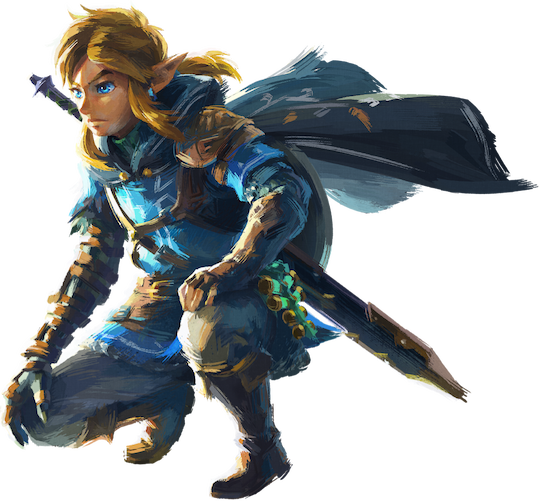
\includegraphics[width=0.5\textwidth]{images/link.png}
\end{center}

\end{frame}

\begin{frame}
\frametitle{Resolving the Links}
The linker combines all executables and makes sure the links are connected to the right places.

The linker also handles referencing shared libraries (e.g., \texttt{glibc}).

We won't focus on how the linker does the job -- that's for the compiler course!

\end{frame}

\part{Executable Organization}

\begin{frame}
\partpage
\end{frame}


\begin{frame}
\frametitle{Minimum Requirements for an Executable}

The executable code that goes in the \texttt{.text} section.

The start symbol/address (\texttt{\_\_start()} which calls \texttt{main()}.

\begin{center}
  
\includegraphics[width=0.3\textwidth]{images/taskmaster.jpg}
\end{center}

\end{frame}

\begin{frame}
\frametitle{Other Sections}

\texttt{.data}: Global or static variables initialized to nonzero values

\texttt{.rodata}: Read-Only data

\texttt{.bss}: Global/static variables initialized to 0. Just reserved space.

\end{frame}

\begin{frame}
\frametitle{So You Want to Run a Program}

A \alert{program} is your compiled code.

A \alert{process} is a program in execution. 

	A process is a program in execution.

	\begin{enumerate}
		\item The instructions and data.
		\item The current state.
		\item Any resources that are needed to execute.
	\end{enumerate}

\end{frame}


\begin{frame}
	\frametitle{Processes vs. Programs}

	Note: two instances of the same program running equals two processes.

	You may have two windows open for Microsoft Word, and even though they are the same program, they are separate processes.


	Similarly, two users who both use Firefox at the same time on a terminal server are interacting with two different processes.

\end{frame}


\begin{frame}
	\frametitle{Two Documents, Two Processes}

	\begin{center}
		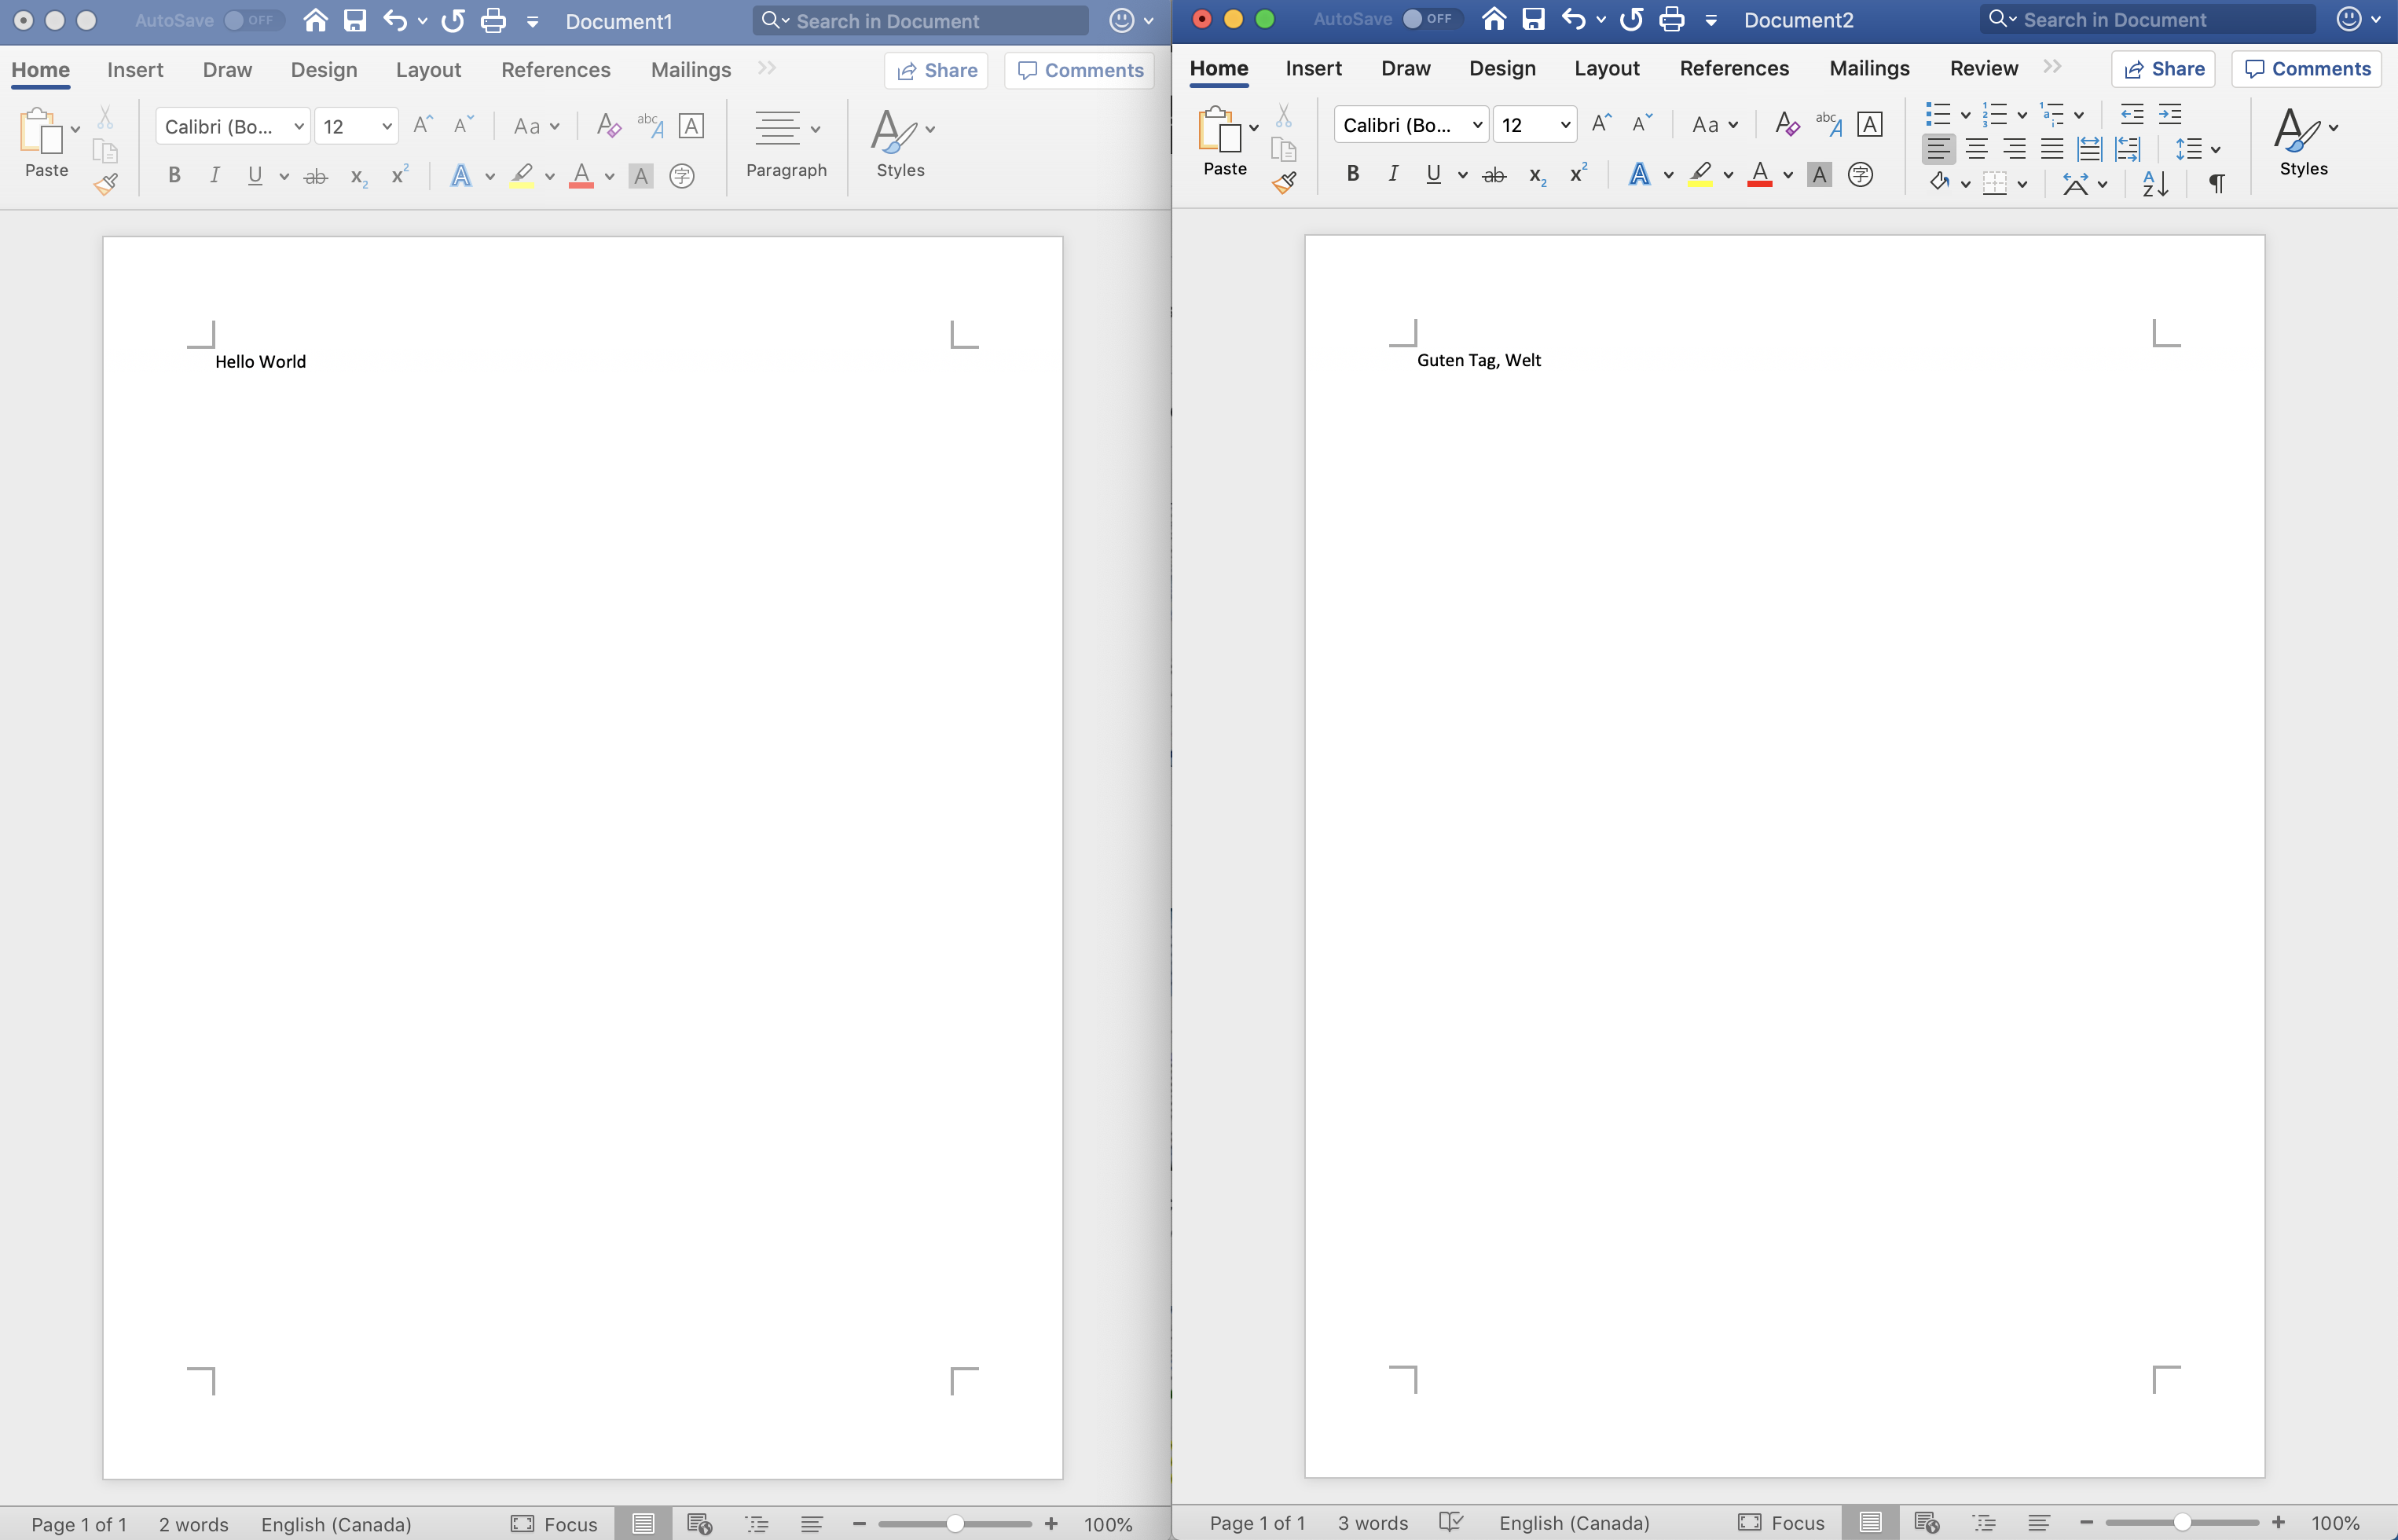
\includegraphics[width=\textwidth]{images/2docs.png}
	\end{center}


\end{frame}

\begin{frame}
\frametitle{Assigning Locations}

At compile time, the compiler resolves static variables/links.

At load-time, the system sets up memory segments and links shared objects.\\
\quad After that, go to the start symbol!

At run-time: resolve dynamic allocation and, oh yes, execute the code.

\end{frame}

\begin{frame}
\frametitle{Executable in Memory}

\begin{center}
  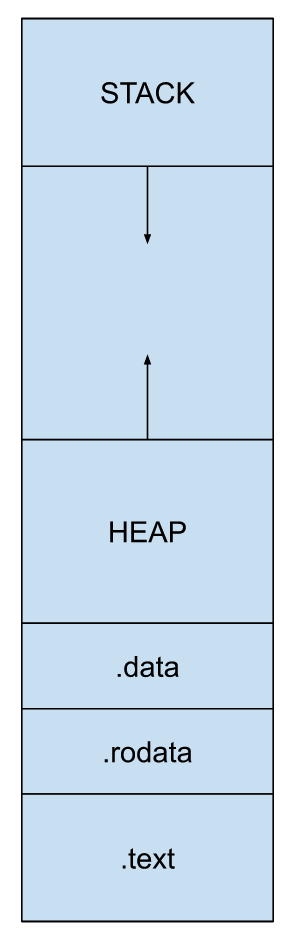
\includegraphics[width=0.22\textwidth]{images/program-in-mem.png}
\end{center}

\end{frame}

\begin{frame}
\frametitle{And Then We Execute}

Once the program is launched, what happens next?

The code runs and does whatever the programmer asked it to do...

Unless the operating system or system needs to step in...\\
\quad But we need to talk more about computer organization first.

\end{frame}

\end{document}

